\documentclass[a4paper,11pt]{book}
%\documentclass[a4paper,twoside,11pt,titlepage]{book}
\usepackage{listings}
\usepackage[utf8]{inputenc}
\usepackage[spanish]{babel}

% \usepackage[style=list, number=none]{glossary} %
%\usepackage{titlesec}
%\usepackage{pailatino}

%\decimalpoint
\usepackage{dcolumn}
\usepackage{float}
\newcolumntype{.}{D{.}{\esperiod}{-1}}
\makeatletter
%\addto\shorthandsspanish{\let\esperiod\es@period@code}
\makeatother


%\usepackage[chapter]{algorithm}
\RequirePackage{verbatim}
%\RequirePackage[Glenn]{fncychap}
\usepackage{fancyhdr}
\usepackage{graphicx}
\usepackage{afterpage}
\usepackage{inputenc}
\usepackage{longtable}

\usepackage[pdfborder={000}]{hyperref} %referencia

% ********************************************************************
% Re-usable information
% ********************************************************************
\newcommand{\myTitle}{Trabajo 3 - Evaluación Continua\xspace}
\newcommand{\myDegree}{MÁSTER EN INVESTIGACIÓN EN INGENIERÍA DE SOFTWARE Y
SISTEMAS INFORMÁTICOS\xspace}
\newcommand{\myName}{César Hugo Bárzano Cruz\xspace}
\newcommand{\myProf}{Nombre Apllido1 Apellido2 (tutor1)\xspace}
\newcommand{\myOtherProf}{Nombre Apllido1 Apellido2 (tutor2)\xspace}
%\newcommand{\mySupervisor}{Put name here\xspace}
\newcommand{\myFaculty}{ Universidad Nacional de Educación a Distancia\xspace}
\newcommand{\myFacultyShort}{UNED-Facultad de informática\xspace}
\newcommand{\myDepartment}{\xspace}
\newcommand{\myUni}{\protect{ Universidad Nacional de Educación a Distancia}\xspace}
\newcommand{\myLocation}{Madrid\xspace}
\newcommand{\myTime}{\today\xspace}
\newcommand{\myVersion}{Version 0.1\xspace}


\hypersetup{
pdfauthor = {\myName hugobarzano@gmail.com},
pdftitle = {\myTitle},
pdfsubject = {},
pdfkeywords = {},
pdfcreator = {LaTeX con el paquete TEXmaker},
pdfproducer = {pdflatex}
}

%\hyphenation{}


%\usepackage{doxygen/doxygen}
%\usepackage{pdfpages}
\usepackage{url}
\usepackage{colortbl,longtable}
\usepackage[stable]{footmisc}
%\usepackage{index}

%\makeindex
%\usepackage[style=long, cols=2,border=plain,toc=true,number=none]{glossary}
% \makeglossary

% Definición de comandos que me son tiles:
%\renewcommand{\indexname}{Índice alfabético}
%\renewcommand{\glossaryname}{Glosario}

\pagestyle{fancy}
\fancyhf{}
\fancyhead[LO]{\leftmark}
\fancyhead[RE]{\rightmark}
\fancyhead[RO,LE]{\textbf{\thepage}}
\renewcommand{\chaptermark}[1]{\markboth{\textbf{#1}}{}}
\renewcommand{\sectionmark}[1]{\markright{\textbf{\thesection. #1}}}

\setlength{\headheight}{1.5\headheight}

\newcommand{\HRule}{\rule{\linewidth}{0.5mm}}
%Definimos los tipos teorema, ejemplo y definición podremos usar estos tipos
%simplemente poniendo \begin{teorema} \end{teorema} ...
\newtheorem{teorema}{Teorema}[chapter]
\newtheorem{ejemplo}{Ejemplo}[chapter]
\newtheorem{definicion}{Definición}[chapter]

\definecolor{gray97}{gray}{.97}
\definecolor{gray75}{gray}{.75}
\definecolor{gray45}{gray}{.45}
\definecolor{gray30}{gray}{.94}

\lstset{ frame=Ltb,
     framerule=0.5pt,
     aboveskip=0.5cm,
     framextopmargin=3pt,
     framexbottommargin=3pt,
     framexleftmargin=0.1cm,
     framesep=0pt,
     rulesep=.4pt,
     backgroundcolor=\color{gray97},
     rulesepcolor=\color{black},
     %
     stringstyle=\ttfamily,
     showstringspaces = false,
     basicstyle=\scriptsize\ttfamily,
     commentstyle=\color{gray45},
     keywordstyle=\bfseries,
     %
     numbers=left,
     numbersep=6pt,
     numberstyle=\tiny,
     numberfirstline = false,
     breaklines=true,
   }

% minimizar fragmentado de listados
\lstnewenvironment{listing}[1][]
   {\lstset{#1}\pagebreak[0]}{\pagebreak[0]}

\lstdefinestyle{CodigoC}
   {
	basicstyle=\scriptsize,
	frame=single,
	language=C,
	numbers=left
   }
\lstdefinestyle{CodigoC++}
   {
	basicstyle=\small,
	frame=single,
	backgroundcolor=\color{gray30},
	language=C++,
	numbers=left
   }


\lstdefinestyle{Consola}
   {basicstyle=\scriptsize\bf\ttfamily,
    backgroundcolor=\color{gray30},
    frame=single,
    numbers=none
   }


\newcommand{\bigrule}{\titlerule[0.5mm]}


%Para conseguir que en las páginas en blanco no ponga cabecerass
\makeatletter
\def\clearpage{%
  \ifvmode
    \ifnum \@dbltopnum =\m@ne
      \ifdim \pagetotal <\topskip
        \hbox{}
      \fi
    \fi
  \fi
  \newpage
  \thispagestyle{empty}
  \write\m@ne{}
  \vbox{}
  \penalty -\@Mi
}
\makeatother

\usepackage{pdfpages}
\begin{document}
\begin{titlepage}
 
 
\newlength{\centeroffset}
\setlength{\centeroffset}{-0.5\oddsidemargin}
\addtolength{\centeroffset}{0.5\evensidemargin}
\thispagestyle{empty}

\noindent\hspace*{\centeroffset}\begin{minipage}{\textwidth}

\centering

\includegraphics[width=0.7\textwidth]{imagenes/Logo-uned.jpg}\\[1.1cm]


{\Huge\bfseries Máster Universitario En Investigación En Ingeniería De Software Y Sistemas Informáticos\\
}
\noindent\rule[-1ex]{\textwidth}{3pt}\\[3.5ex]
{\large\bfseries Generación Automática de Código}
\end{minipage}

\vspace{2.5cm}
\noindent\hspace*{\centeroffset}\begin{minipage}{\textwidth}
\centering

\textbf{Autor}\\ {César Hugo Bárzano Cruz}\\[2.5ex]


\includegraphics[width=0.3\textwidth]{imagenes/Logo-master.png}\\[0.1cm]
\textsc{Trabajo de Investigación}\\
\textsc{---}\\
2017/2018
\end{minipage}
%\addtolength{\textwidth}{\centeroffset}
%\vspace{\stretch{2}}
\end{titlepage}




%\frontmatter
\tableofcontents
\listoffigures
%\listoftables

%
%\mainmatter
%\setlength{\parskip}{5pt}

%\input{capitulos/01_Introduccion}


\chapter{Resumen}

En el dominio de la WEB 2.0 el nuevo modelo de desarrollo al que tienden las empresas se basa en metodologías agile, donde se premia la rápida entrega de pequeñas funcionalidades junto con iteraciones mas seguidas con los equipos. Es común la creación de pequeños servicios, con funcionalidad muy especifica para cubrir cierta necesidad de negocio y ademas de una manera dinámica y volátil. Esto puede suponer una carga de trabajo importante para los equipos de desarrollo, pues ademas de mantener los servicios funcionales han de crear nuevos constantemente, por este motivo se propone el siguiente trabajo basado en la generación dinámica de servicios web.  La idea de este generador es la de reducir el tiempo de desarrollo de nuevos servicios procurando al desarrollardor de un esqueleto o scafolding funcional de un modelo de negocio muy concreto. La generación automática de servicios también puede resultar muy útil en el campo de la formación o capacitación ya que puede proporcionar el proyecto o estructura base para que el capacitador pueda mostrar los conceptos importantes en el desarrollo de servicios web a los alumnos o técnicos que reciban dicha capacitación.  


El objetivo de esta investigación es el de automatizar mediante técnicas de generación automática de código la generación de servicios web base REST.  El resultado de esta investigación serán un generador de servicios web en distintos lenguajes, así como un pequeño caso de uso a modo de conjunto de pruebas automáticas que permita validar el correcto funcionamiento del servicio generado. 
 
\chapter{Introducción}

En los últimos años, la WEB 2.0 ha evolucionado de manera veloz debido a la gran demanda de infomación que tanto usuario como empresa han generado con el uso de las nuevas tecnologías. El desarrollo de aplicaciones web basadas en servicios ha marcado un antes y un después, haciendo que los datos tomen un nuevo valor. La transformación digital es un hecho que esta cambiado el modo en que las empresas y usuarios interactuan con la información puesto que el acceso a los datos facilita la toma de decisiones, datos que hasta hace unos años no se pensaba que tendrían el valor social y económico que tienen hoy en día. Es notable como la información y los canales de comunicación crecen día a día satisfaciendo necesidades encubiertas que el usuario no conocía, automatizando procesos de negocio y mejorando tareas de gobierno.  


El desarrollo de aplicaciones web normalmente va asociado a procesos de desarrollo ágil donde se premia la alta disponibilidad, la rápida creación y la integración de nuevos servicios de información con los ya disponibles. Estas metodologías son responsables en su justa medida del rápido crecimiento de lo denominado WEB 2.0 o infraestructura de información distribuida a la cual, todos podemos acceder con los innumerables dispositivos que nos rodean. 

Estas metodologías, con aspectos muy beneficiosos para el ingeniería del software, tienen ciertas carencias con respecto a las metodologías de desarrollo tradicional. Si por un momento, dejamos de lado las tecnologías de la información y nos centramos en otros sectores  donde el software cumple un papel vital, como por ejemplo proyectos en el ámbito espacial, defensa, automoción o aeronáutica, las lineas de desarrollo ágil son rechazadas por completo, puesto que el software resultante de estos proyectos ha sido validado y testeado durante largos años, sometidos a  largos procesos de calidad y pruebas, procesos muy costo y lento para ser aplicado en el desarrollo de aplicaciones web o servicios cloud. 

La gran demanda de información y soluciones cloud en ocasiones puede ocasionar ciertos problemas ya que se disponibilizan servicios o versiones cuyo estado no es fiable, bajo el escudo de que los servicios de la información son de carácter volátil.  Esta demanda produce una gran cantidad de software que ha de ser mantenido y actualizado, tarea complicada de manejar si se tiene en cuenta que cada solución puede ser implementada por  distintos equipos, con distintos lenguajes de programación o tecnologías.  Es aquí donde la generación automática de código marca la diferencia. Como se verá en los siguientes capítulos se propone la implementación de un generador de servicios cloud basados en REST cuyo objetivo sea la unificación del desarrollo de servicios. Dando un punto común y estructura base que permita a los desarrolladores avanzar rápidamente, produciendo de esta forma productos software de similar estructura, aunque desarrollen con distintas tecnologías. 



Para ello, con el foco en el desarrollo ágil de aplicaciones se va a plantear una solución a como los servicios de la información han de exponerse al mundo, garantizando que su resultado final es el esperado aplicando tecnicas de validación tradicional a los procesos de desarrollo ágil, siendo aquí donde la generación automática de código desempeñará un papel fundamental, ya que se intentará automatizar el proceso generativo del plan de validación de estos servicios. De esta manera, la solución final, verificará el desarrollo de aplicaciones sin incluir la dilatión en el tiempo que conlleva la ejecución de un plan de validación completo sobre un proyecto software.    

\chapter{El Problema}

El desarrollo basado en metodologías agiles  principalmente va enfocado a proyectos que precisan de una especial rapidez y flexibilidad en su proceso. En muchas ocasiones son proyectos relacionados con el desarrollo de software o el mundo de internet. En sectores constantemente cambiantes, las organizaciones necesitan desarrollar sus servicios rápidamente para ser altamente competitivos, y esto no es tarea fácil. Muchas veces es necesario ir probando las distintas funcionalidades del servicio sobre la marcha y medir si está funcionando o no para acabar ofreciendo una solución final.

Si se utilizan metodologías  de desarrollo tradicionales, estas revisiones (o tests) pueden suponer un retraso en las fechas de entrega, aumento de costes y del volumen de trabajo. Además, también podría suceder que para cuando se tenga el producto final éste ya quede obsoleto. He aquí la importancia del  desarrollo Agile. 

Las metodologías ágiles se basan en un enfoque flexible. Los miembros del equipo trabajan en pequeñas fases y equipos sobre actualizaciones concretas del producto. Después, se prueba cada actualización en función de las necesidades del cliente. El producto final de un proyecto ágil puede perfectamente ser distinto al que se había previsto inicialmente. No obstante, durante los procesos de pruebas se sigue trabajando según los requerimientos del cliente, de forma que el producto final sigue respondiendo a sus necesidades. En las siguientes secciones se abordarán las metodologías agile mas comunes y como afectan al desarrollo de servicios cloud bajo  arquitecturas basadas en microservicios, y como la generación automática de código desempeña un gran papel. 


\section{Metodologías Ágiles}
\subsubsection{Scrum}

Scrum es un proceso en el que se aplican de manera regular un conjunto de buenas prácticas para trabajar colaborativamente, en equipo, y obtener el mejor resultado posible de un proyecto. Estas prácticas se apoyan unas a otras y su selección tiene origen en un estudio de la manera de trabajar de equipos altamente productivos.

En Scrum se realizan entregas parciales y regulares del producto final, priorizadas por el beneficio que aportan al receptor del proyecto. Por ello, Scrum está especialmente indicado para proyectos en entornos complejos, donde se necesita obtener resultados pronto, donde los requisitos son cambiantes o poco definidos, donde la innovación, la competitividad, la flexibilidad y la productividad son fundamentales.

\begin{figure}[H]  
\centering 
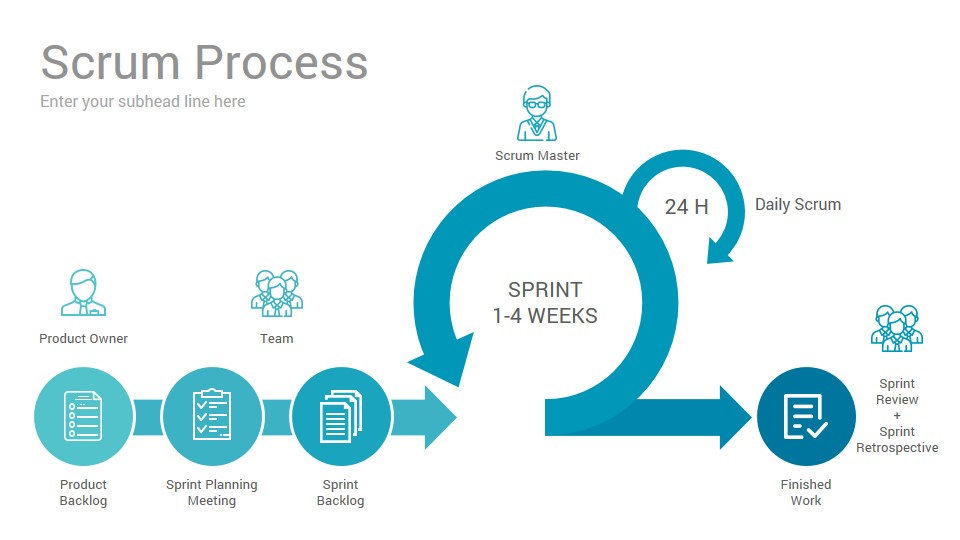
\includegraphics[scale=0.35]{imagenes/scrum.jpg}
\caption{ Scrum Process\cite{scrum} }  
\end{figure}


\subsubsection{Kanban}

La metodología Kanban es una manera de gestionar el trabajo de forma fluida. La palabra Kanban proveniente de Japón, es un símbolo visual que se utiliza para desencadenar una acción. A menudo se representa en un tablero Kanban para reflejar los procesos de su flujo de trabajo.

\begin{figure}[H]  
\centering 

\includegraphics[scale=0.35]{imagenes/kamban.jpg}
\caption{ Kamban Table\cite{kanban} }  
\end{figure}

\subsubsection{Lean}
Lean son una serie de principios enfocados a eliminar todas las tareas que no aporten valor sobre aquello que estamos realizando. Aplicado a un proyecto, aquello que no aporte valor al producto o servicio final. Para ello, visualiza todo todo el proceso que se produce en una cadena de valor a lo largo de un proyecto y, en todos aquellos puntos que se produce desperdicio, lo elimina.

\begin{figure}[H]  
\centering 
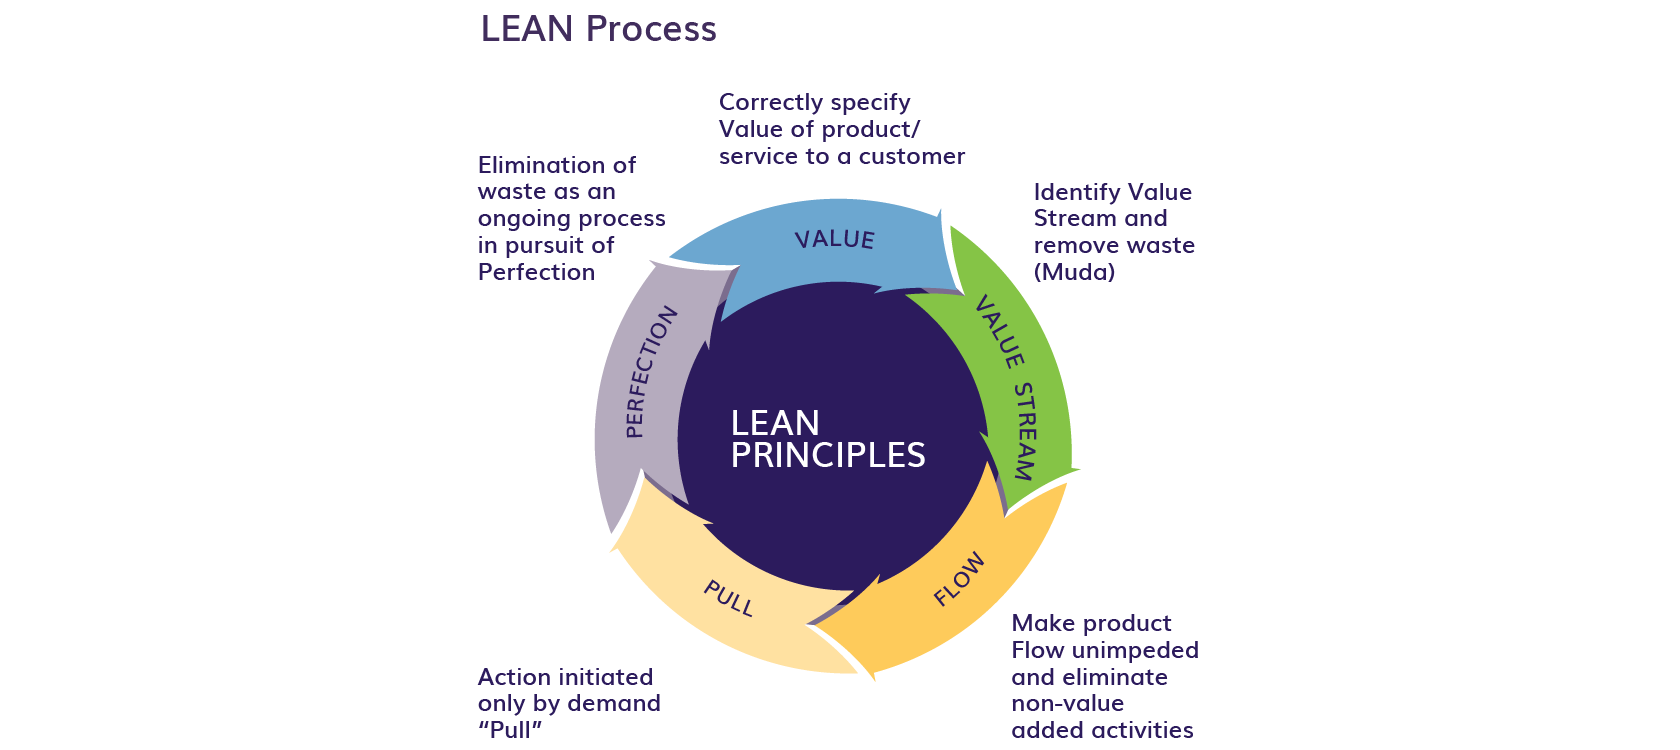
\includegraphics[scale=0.35]{imagenes/lean.png}
\caption{ Lean Process\cite{lean} }  
\end{figure}

\subsubsection{XP Programming}
La programación extrema o eXtreme Programming (XP) es un enfoque de la ingeniería de software formulado por Kent Beck, autor del primer libro sobre la materia, Extreme Programming Explained: Embrace Change\cite{xp}

Es una metodología ágil centrada en potenciar las relaciones interpersonales como clave para el éxito en desarrollo de software, promoviendo el trabajo en equipo, preocupándose por el aprendizaje de los desarrolladores, y propiciando un buen clima de trabajo. XP se basa en realimentación continua entre el cliente y el equipo de desarrollo, comunicación fluida entre todos los participantes, simplicidad en las soluciones implementadas y coraje para enfrentar los cambios. XP se define como especialmente adecuada para proyectos con requisitos imprecisos y muy cambiantes, y donde existe un alto riesgo técnico.

\begin{figure}[H]  
\centering 
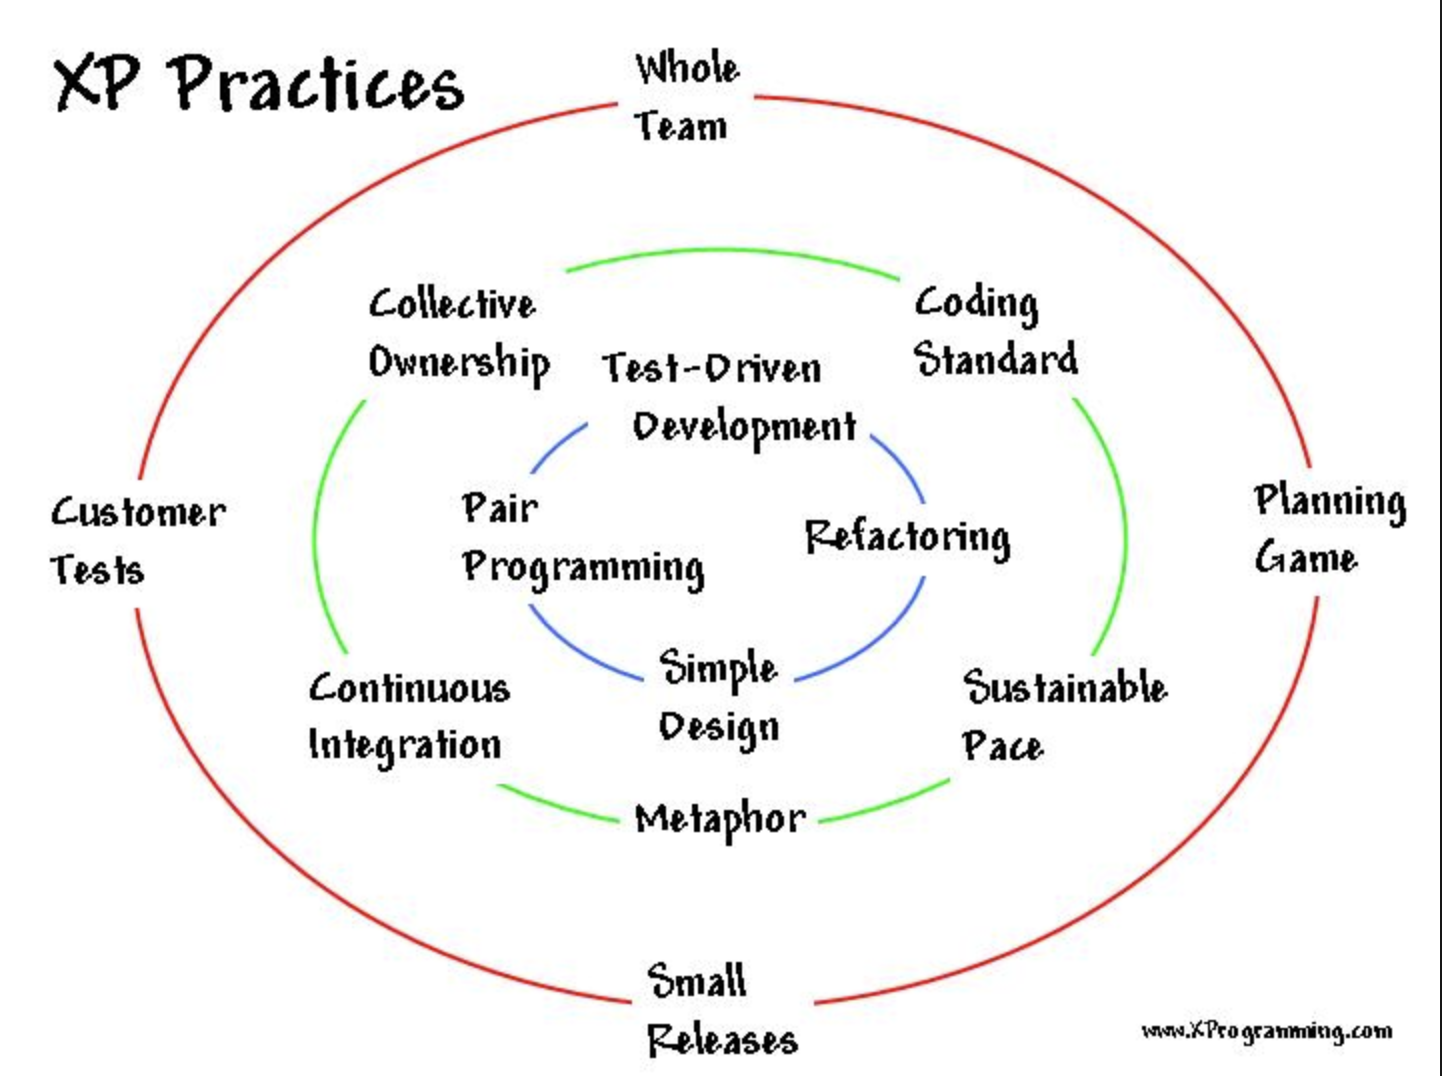
\includegraphics[scale=0.35]{imagenes/xp.png}
\caption{ XP Practices\cite{xp2} }  
\end{figure}


.  

\section{Servicios web: REST}

La Transferencia de Estado Representacional (REST - Representational State Transfer) fue ganando amplia adopción en toda la web como una alternativa más simple a SOAP y a los servicios web basados en el Lenguage de Descripción de Servicios Web (Web Services Descripcion Language - WSDL). 

REST define un set de principios arquitectónicos por los cuales se diseñan servicios web haciendo foco en los recursos del sistema, incluyendo cómo se accede al estado de dichos recursos y cómo se transfieren por HTTP hacia clientes escritos en diversos lenguajes. Los 4 principios de REST son: 

\begin{enumerate}
\item Utiliza los métodos o verbos HTTP de manera explícita
\item No mantiene estado
\item Expone URIs
\item Transfiere XML, JavaScript Object Notation (JSON), o ambos
\end{enumerate}

\subsection{Arquitecturas Basadas en micro-servicios}

El enfoque tradicional sobre el desarrollo de aplicaciones se centró en el monolito, donde todas las partes de la aplicación que se pueden implementar están contenidas en esa única aplicación. Esto tiene sus desventajas: cuanto más grande es la aplicación, más difícil resulta solucionar problemas nuevos y agregar funciones nuevas con rapidez. Un enfoque basado en los microservicios para el diseño de las aplicaciones resuelve estos problemas e impulsa el desarrollo y la capacidad de respuesta.

Los microservicios se pueden considerar tanto un tipo de arquitectura como un modo de programar software. Con los microservicios, las aplicaciones se dividen en sus componentes más pequeños e independientes entre sí. A diferencia del enfoque tradicional y monolítico de las aplicaciones, en el que todo se integra en una única pieza, los microservicios son independientes y funcionan en conjunto para llevar a cabo las mismas tareas. Cada uno de estos elementos o procesos es un microservicio. Este enfoque sobre el desarrollo de software privilegia el nivel de detalle, la sencillez y la capacidad de compartir procesos similares en varias aplicaciones. Es un componente fundamental de la optimización del desarrollo de aplicaciones hacia un modelo nativo de la nube.

\begin{figure}[H]  
\centering 
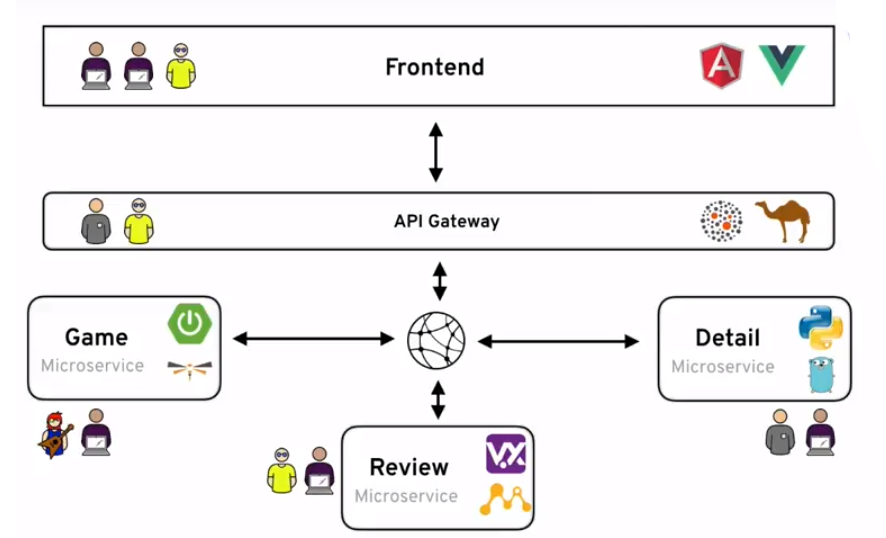
\includegraphics[scale=0.35]{imagenes/micro.png}
\caption{ Arquitectura Basada en Microservicios\cite{micro} }  
\end{figure}

\section{GAC en Servicios Web}

De las distintas metodológias ágiles utilizadas en el proceso de desarrollo de servicios web, se pone de manifiesto que el objetivo es cubrir rápidamente la demanda de nuevas funcionalidades o features que no estaban previstas inicialmente, evolucionando bajo demanda del cliente final e iterando con pequeñas entregas del producto. Por otro lado, se ha visto que la arquitectura orientada a microservicios esta ligada a este tipo de productos e intenta descomponer en la medida de lo posible todas las funcionalidades o recursos rompiendo con las arquitecturas monolíticas tradicionales y mostrando el producto o sistema final como la suma de muchas piezas pequeñas que cumplen una funcionalidad concreta. Es aquí donde la generación automática de código puede marcar la diferencia, ya que ante la demanda de nuevas funcionalidades es preferible la creación ( o generación) de nuevas piezas que intenten resolver el problema concreto de la manera más atómica posible. 

Para ello, se propone en este trabajo la implementación de un generador de servicios web basado en REST que permita a los equipos de desarrollo generar nuevas funcionalidades asegurando que el código de los servicios generados sea todo lo genérico que se pueda, de manera que las reglas de codificación, Apis, estructura de los proyectos, separación entre capaz, acceso a base de datos, pruebas y en general toda funcionalidad base esperada por un servició web  sea proporcionada por el generador de manera automática, transversal y común. 





\chapter{Desarrollo de la práctica }

Visto el enunciado del problema en el capítulo anterior, se propone la implementación de un generador de servicios web basados en REST. 

\section{Recursos de programación utilizados}

El generador ha sido desarrollado mediante el lenguaje de programación GO\cite{go}.  Go es un lenguaje de programación inspirado en C, compilado, estáticamente tipado, concurrente y con un enfoque de programación orientada a objetos.  Principales características de GO:

\begin{enumerate}
\item Compilado: No es necesario instalar ningún programa para que el programa desarrollado funcione en el sistema operativo para el que se compiló. 
\item Estáticamente Tipado: Las variables son tipadas de manera estática, así que si la variable x se define como entera, será entera durante todo su alcance.
\item Concurrente: Está inspirado en CSP - Communicating sequential processes\cite{csp}
\item Uso de paquetes: Usa paquetes para organizar el código.
\end{enumerate}

El generador propuesto es capaz de generar servicios web en el lenguaje de programación GO y también en el lenguaje de programación Javascript\cite{js} haciendo uso del framework NODE. JavaScript es un lenguaje de programación interpretado. Se define como orientado a objetos, basado en prototipos, imperativo, débilmente tipado y dinámico. Node\cite{node} ( node.js)  es un entorno de ejecución para JavaScript construido con el motor de JavaScript V8 de Chrome.

De manera adicional y con el objetivo de validar que efectivamente el código generado para el servicio es correcto, el generador también produce una caso de uso básico en el que probar las capacidades CRUD(Create, Read, Update and Delete) del servicio. Para ello, el generador producirá un caso de uso en lenguaje de scripting BASH\cite{bash} donde usando la instrucción cURL\cite{curl} se automatizarán distintas peticiones HTTP al servicio generado. 

Finalmente para la confección de esta memoria se ha utilizado LaTEX con el paquete de librerías texlive-full y el editor texmaker. Los siguientes enlaces muestran como instalar y utilizar correctamente LaTEX, han sido utilizados como referencia para el presente documento. 

\begin{enumerate}
\item \href{http://milq.github.io/install-latex-ubuntu-debian/}{Instalar LaTeX}
\item \href{ http://minisconlatex.blogspot.com.es/}{Usar LaTeX}
\end{enumerate}


\section{Especificación de la solución}

El generador puede ser encontrado en el siguiente repositorio de Github \href{ https://github.com/hugobarzano/restandtestgenerator}{hugobarzano/restandtestgenerator} el código relativo al generador será entregado como parte del trabajo de investigación, pero para facilitar la comprensión de las partes que forman el generador, se hará referencia a dicho repositorio de GitHub. 

A grandes rasgos, en una ejecución nominal del generador, se leerán todos los ficheros que se encuentren en el directorio  \href{https://github.com/hugobarzano/restandtestgenerator/tree/master/input}{input/}. Por cada uno de los ficheros de este directorio, el generador producirá el código funcional correspondiente a un servicio web en GO y en NODE. De manera adicional, se generará un caso de prueba donde se realizaran peticiones a la API generada mediante Shell scripting.  El siguiente bloque muestra un ejemplo de configuración, correspondiente al fichero de ejemplo  \href{https://github.com/hugobarzano/restandtestgenerator/blob/master/input/cats\_cloud\_service.json}{restandtestgenerator/input/cats\_cloud\_service.json}. 

\begin{lstlisting}[language=python,caption={ Ejemplo Entrada Generador }]
[{
  "name": "Miauuu as a service",
  "service": "/cats",
  "url": "http://localhost",
  "port":":8080",
  "body": {
    "name":"Wurst",
    "alias": "Mi bolita gatita bonita",
    "reina": true,
    "age": 1.5,
    "color": "Negro como mi alma"
  }
}]
\end{lstlisting}


Los campos correspondientes al ejemplo de configuración representan: 

\begin{enumerate}
\item "name": Nombre común del servicio.
\item "service": Api generada donde se expondrá el servicio.
\item "url":  Host donde se probará el servicio.
\item "port": Puerto donde el servicio será expuesto.
\item "body": Representa el modelo de negocio o modelo de datos. Es la entidad que el servicio será capaz de manejar.  Los datos de ejemplo dados serán usados en la generación de las pruebas. 
\end{enumerate}

\subsection{Comportamiento de la Solución}

En la siguiente sección dedicada a Pruebas se ejemplificará el comportamiento del generador mediante unos casos de prueba. De manera literal, el generador cargará los ficheros de configuración ( directorio input) para cada uno de estos ficheros que especifican un servicio web: 

\begin{enumerate}
\item El generador producirá el Scaffolding o estructura base del servicio GO.
\item El generador producirá el Scaffolding o estructura base del servicio NODE.
\item  El generador producirá el Modelo de negocio y la configuración necesaria para la base de datos del servicio GO.
\item El generador producirá el modelo de negocio para el servicio NODE.
\item El generador producirá el TestCase relativo al servicio generado. El Test Case será producido en shell scripting por lo que puede ser independientemente ejecutado contra cualquiera de las tecnologías con las que el servicio es generado.
\end{enumerate}

\section{Alcance y Limitaciones}

El generador propuesto es capaz de generar servicios funcionales en GO y en NODE. Los servicios generados están constituidos por una API REST CRUD que soporta los verbos http: GET, POST, PUT, DELETE.  El modelo de negocio generado para el servicio es dinámico. El Generador produce toda la configuración necesaria para la capa de persistencia. El generador produce todas las dependencias necesarias para la correcta ejecución del servicio. El generador produce un caso de uso que permite validar el correcto funcionamiento del servicio generado. 

Por otra parte, el generador solo soporta tipos de dato String, Number y Boolean, podría ser extendido mediante un JsonSchema para aceptar tipos de datos y objetos complejos. La capa de persistencia de los servicios generados es mongoDB, es decir, están acoplados a este tipo de tecnología, podría ser extendido para soportar distintas tecnologías como capa de persistencia. El generador solo produce servicios en Go y NODE, podría ser extendido para generar servicios en Python. El generador podría utilizar algún framework de testing para generar más pruebas para los servicios. 

\section{Pruebas}

En esta Sección, se plantean distintos escenarios con el objetivo de mostrar el comportamiento del generador ante distintos casos. Se realizará un total de 4 escenarios distintos. El código generado formará parte de la entrega. 


\subsection{Escenario 1: People Service}

En este escenario se va a generar el siguiente servicio:

\begin{lstlisting}[language=python,caption={ Ejemplo Entrada Generador: people.json }]
[{
  "name": "People for your bushiness",
  "service": "/people",
  "url": "http://localhost",
  "port":":8080",
  "body": {
    "name":"John Smith",
    "company": "CesarCorp",
    "job": "develop",
    "city": "CDMX"
  }
}]
\end{lstlisting}

Básicamente consiste en una API para disponibilizar información sobre los empleados de una empresa. Como se puede observar, el modelo de negocio de este servicio está formado íntegramente por strings.
En este escenario el análisis se centrará en mostrar el código GO generado, su ejecución y posteriormente validación con el propio test generado. Para ello, es necesario guardar la entrada arriba indicada en un fichero denominado people.json dentro del directorio input/ del proyecto. Una ves establecida la entrada en el directorio necesario, es necesario ejecutar el generador usando el ejecutable adecuado para la plataforma sobre la que se realicen las pruebas, en este caso MAC: 

\begin{lstlisting}[language=python,caption={ Ejemplo Entrada Generador: people.json }]
\$  ./restandtestgenerator.darwin 
\end{lstlisting} 

Tras la ejecución, en el directorio output/ se ha generado el siguiente contenido:

\begin{figure}[H]  
\centering 
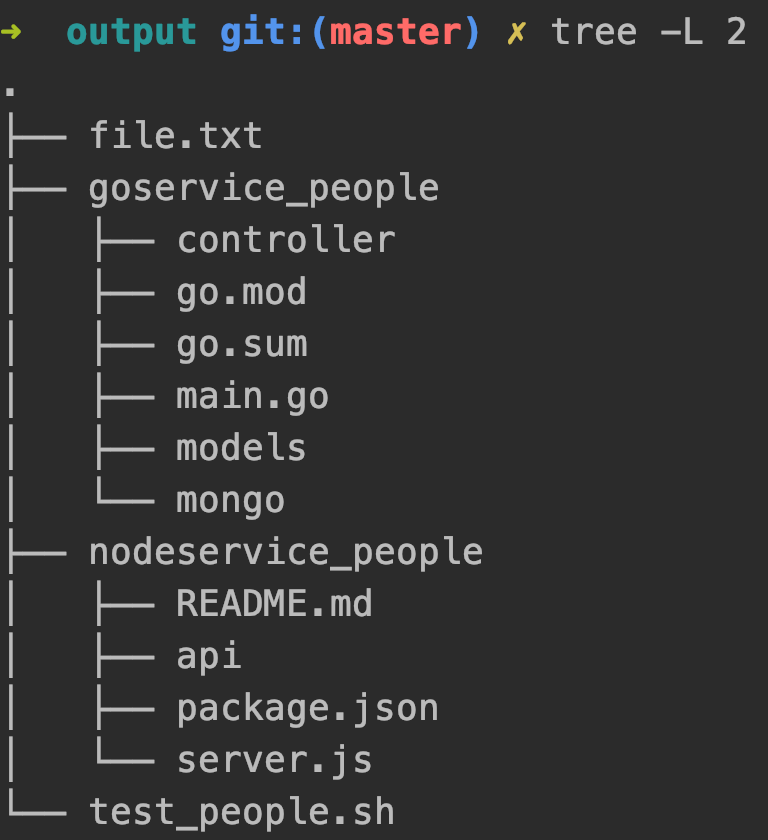
\includegraphics[scale=0.35]{imagenes/t11.png}
\caption{ Servicio generado people.json}  
\end{figure}

Como se puede observar, se ha generado el servicio Go, el servicio NODE y el test\_case.sh. En este escenario se va a poner el foco en goservice\_people. La estructura generada es la siguiente:

\begin{figure}[H]  
\centering 
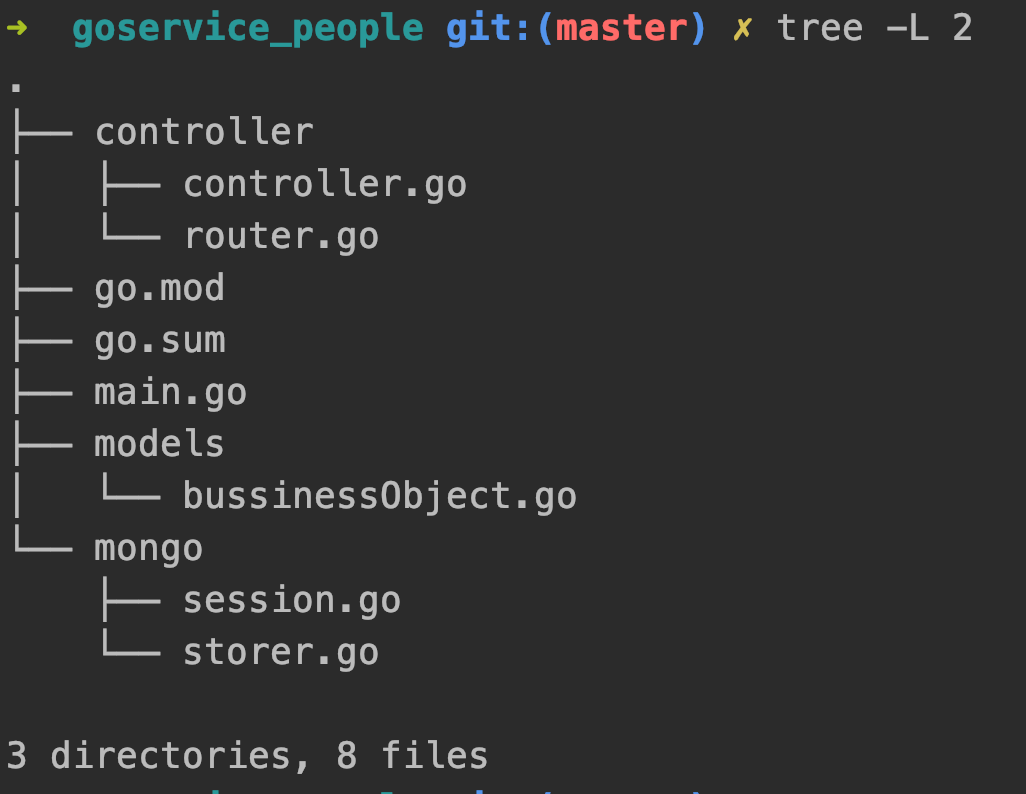
\includegraphics[scale=0.35]{imagenes/t12.png}
\caption{ Servicio generado people.json}  
\end{figure}

Se pueden apreciar los siguientes paquetes:

\begin{enumerate}
\item controller: Encargado de todo lo relacionado con la API del servicio
\item models: Donde el modelo de negocio toma entidad
\item mongo: Paquete responsable de la comunicación con la capa de persistencia
\item main.go: Programa principal
\item ficheros go.mod y go.sum: Lugar en el que se especifican las dependencias del servicio
\end{enumerate}

Para ejecutar el servicio generado /people seria necesario: 


\begin{lstlisting}[language=python,caption={ Ejemplo Ejecución /people }]
\$  cd output/goservice_people
\$ go run main.go
\end{lstlisting} 

\begin{figure}[H]  
\centering 
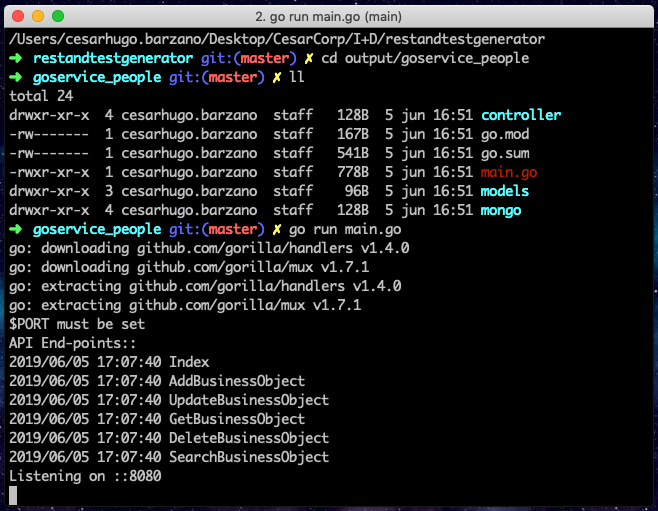
\includegraphics[scale=0.35]{imagenes/t13.png}
\caption{ Ejemplo Ejecución /people}  
\end{figure}

De manera adicional, el generador ha producido el siguiente test\_people.sh para el escenario:

\begin{lstlisting}[language=python,caption={  test\_people.sh }]
#!/usr/bin/env bash

TestStep_1() {
echo "----- Test Step - 1 -----"
echo "TEST STEP - 1 "
echo "API NAME: People for your bushiness"
echo "URL: http://localhost:8080/people"
echo "Scripting field..."
#<<SCRIPT_PLACEHOLDER>>

response_code=$(curl -XPOST -i -k "http://localhost:8080/people" --write-out %{http_code} --output /dev/null -d  '{"city":"CDMX","company":"CesarCorp","job":"develop","name":"John Smith"}' )

if [ $response_code = "201" ]; then
    echo "STEP - 1: PASS"
    echo "----- --- -----"
    return 0
else
  echo "STEP - 1: FAIL"
  return 1
fi

}

TestStep_2() {
echo "----- Test Step - 2 -----"
echo "TEST STEP - 2 "
echo "API NAME: People for your bushiness"
echo "URL: http://localhost:8080/people"
echo "Scripting field..."
get=$(curl -sb -H "Accept: application/json" "http://localhost:8080/people" | jq '.[0]._id')  
  export ID=$get

response_code=$(curl -XGET -i -k --write-out %{http_code} --output /dev/null http://localhost:8080/people)

if [ $response_code = "200" ]; then
    echo "STEP - 2: PASS"
    echo "----- --- -----"
    return 0
else
  echo "STEP - 2: FAIL"
  return 1
fi

}

TestStep_3() {
echo "----- Test Step - 3 -----"
echo "TEST STEP - 3 "
echo "API NAME: People for your bushiness"
echo "URL: http://localhost:8080/people"
echo "Scripting field..."
#<<SCRIPT_PLACEHOLDER>>

response_code=$(curl -XPUT -i -k "http://localhost:8080/people/${ID//\"}" --write-out %{http_code} --output /dev/null -d  '{"city":"CDMX_Update","company":"CesarCorp_Update","job":"develop_Update","name":"John Smith_Update"}' )

if [ $response_code = "200" ]; then
    echo "STEP - 3: PASS"
    echo "----- --- -----"
    return 0
else
  echo "STEP - 3: FAIL"
  return 1
fi

}

TestStep_4() {
echo "----- Test Step - 4 -----"
echo "TEST STEP - 4 "
echo "API NAME: People for your bushiness"
echo "URL: http://localhost:8080/people"
echo "Scripting field..."
echo $ID

response_code=$(curl -XDELETE -i -k --write-out %{http_code} --output /dev/null http://localhost:8080/people/${ID//\"})

if [ $response_code = "200" ]; then
    echo "STEP - 4: PASS"
    echo "----- --- -----"
    return 0
else
  echo "STEP - 4: FAIL"
  return 1
fi

}

TEST_PASS=0
TEST_FAIL=0
TOTAL_TEST=0

declare -a arr=("TestStep_1" "TestStep_2" "TestStep_3" "TestStep_4" )

for i in "${arr[@]}"
do
    if $i; then
        TEST_PASS=$((TEST_PASS+1));
    else
        TEST_FAIL=$((TEST_FAIL+1));
fi
done

echo "--- TEST CASE REPORT ---"
echo "TEST PASS: " $TEST_PASS
echo "TEST FAIL: " $TEST_FAIL
echo "TOTAL EXECUTED: " ${#arr[@]}
echo "--- --- --- --- --- ---"
\end{lstlisting} 

Dicho test puede ser ejecutado contra el actual servicio en ejecución de la siguiente manera:


\begin{lstlisting}[language=python,caption={  exec test\_people.sh }]
chmod +x test_people.sh
./test_people.sh
\end{lstlisting} 

El resultado de dicha ejecución valida que el servicio generado funciona correctamente:


\begin{figure}[H]  
\centering 
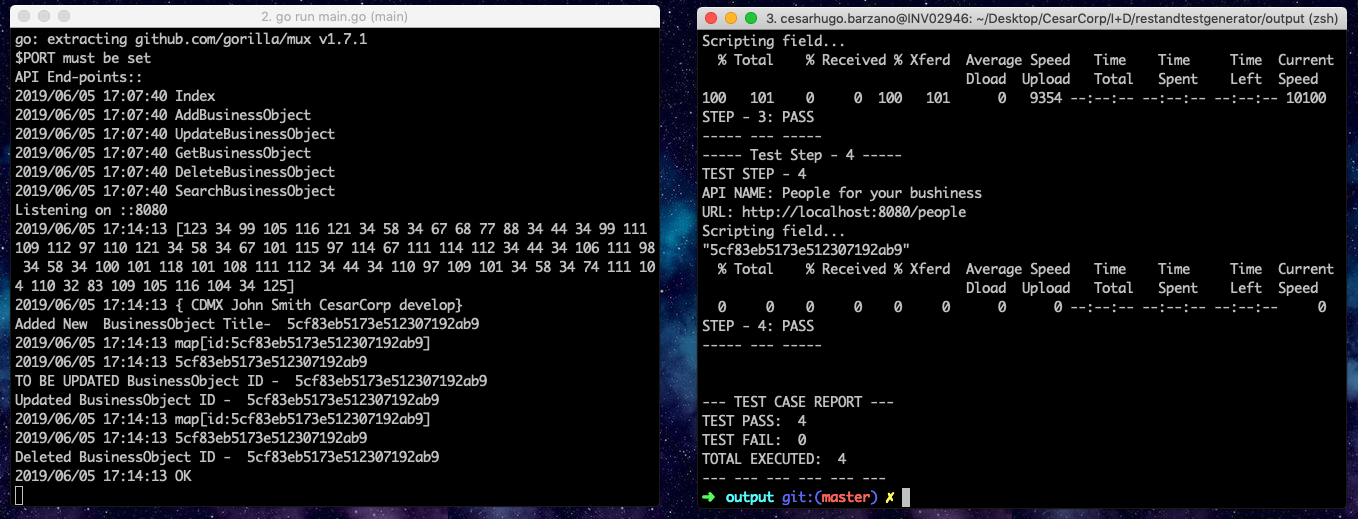
\includegraphics[scale=0.25]{imagenes/t14.png}
\caption{ test\_people.sh result}  
\end{figure}

\subsection{Escenario 2: Players Location}

En este escenario, se va a generar el servicio /location capaz de manejar las posiciones de jugadores en un sistema de coordenadas, de gran utilidad por ejemplo en el back-end de juegos móviles. El objeto de este escenario es mostrar la capacidad del generador para generar objetos de negocio tipo numérico. De manera adicional, en este escenario se hará foco en el servicio NODE generado. El servicio generado en cuestión es:

\begin{lstlisting}[language=python,caption={ Ejemplo Entrada Generador: location\_api.json }]
[{
  "name": "Players location",
  "service": "/location",
  "url": "http://localhost",
  "port":":8080",
  "body": {
    "player":"suave93",
    "x": 67.33,
    "y": 45.66,
    "z": 5.55
  }
}]
\end{lstlisting}

Para ello, es necesario guardar esta especificación de servicio en un fichero denominado location\_api.json dentro del directorio input y ejecutar el generador:

\begin{lstlisting}[language=python,caption={ Ejemplo Ejecución Generador: location\_api.json }]
\$  ./restandtestgenerator.darwin 
\end{lstlisting} 

Tras la ejecución, en el directorio output/ se ha generado el siguiente contenido:

\begin{figure}[H]  
\centering 
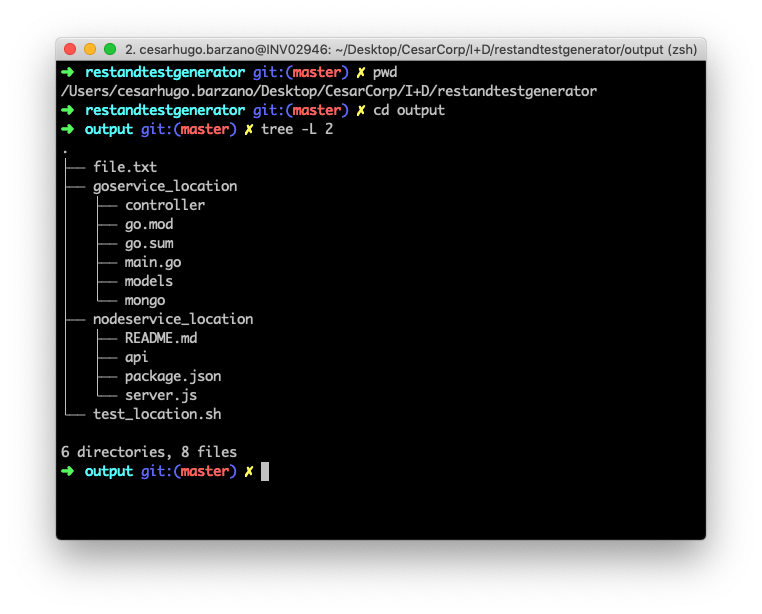
\includegraphics[scale=0.35]{imagenes/t21.png}
\caption{ Servicio generado location\_api.json}  
\end{figure}

Como se puede observar, se ha generado el servicio Go, el servicio NODE y el test\_case.sh. En este escenario se va a poner el foco en nodeservice\_location. La estructura generada es la siguiente:

\begin{figure}[H]  
\centering 
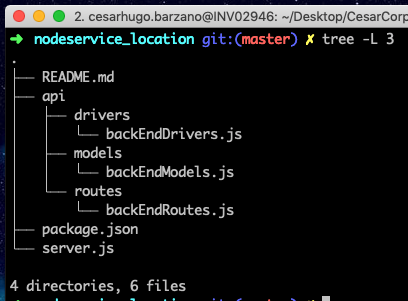
\includegraphics[scale=0.35]{imagenes/t22.png}
\caption{ Servicio generado location\_api.json}  
\end{figure}

Se pueden apreciar los siguientes modulos:

\begin{enumerate}
\item api/drivers: Contiene el código necesario para la comunicación con la capa de persistencia
\item api/models: Contiene el modelo de negocio generado para el servicio
\item routes: Contiene el código de la API del servicio
\item server.js: Fichero principal del servidor de aplicaciones
\item package.json: Ficho de dependencias. Pendiente de inicializar. 
\end{enumerate}


Para inicializar el servicio NODE  /location seria necesario ejecutar y contestar a las preguntas de npm: 

\begin{lstlisting}[language=python,caption={ Ejemplo inicialización /location }]
\$  npm init
{
  "dependencies": {
    "body-parser": "~1.18.2",
    "express": "~4.16.2",
    "mongoose": "^5.4.15",
    "package.json": "^2.0.1"
  },
  "devDependencies": {
    "nodemon": "^1.18.10"
  },
  "scripts": {
    "start": "node server.js"
  },
  "name": "nodeservice_location",
  "description": "",
  "version": "1.0.0",
  "main": "server.js",
  "author": "",
  "license": "ISC"
}
\end{lstlisting} 

Para instalar las dependencias que el servicio NODE necesita: 

\begin{lstlisting}[language=python,caption={ Ejemplo instalación /location }]
$ npm install
\end{lstlisting} 

Para ejecutar el servicio NODE: 

\begin{lstlisting}[language=python,caption={ Ejemplo Ejecución /location }]
$ npm start
\end{lstlisting} 

\begin{figure}[H]  
\centering 
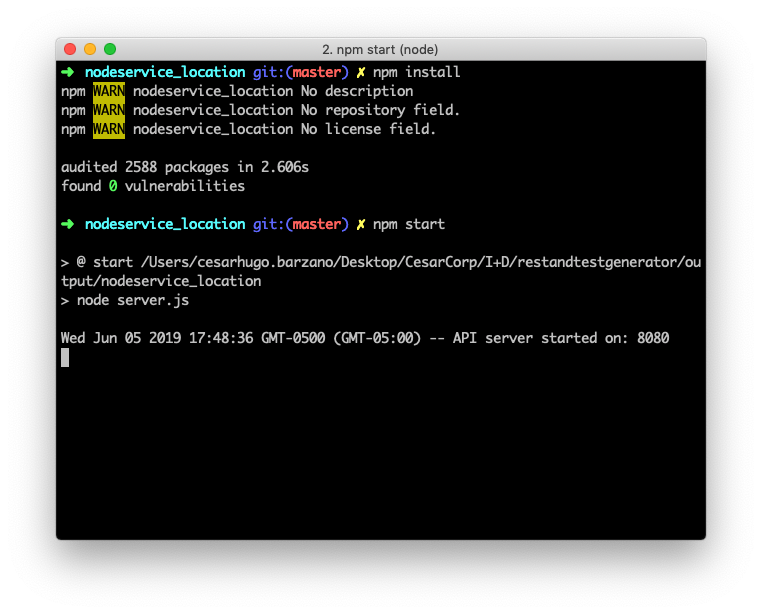
\includegraphics[scale=0.35]{imagenes/t23.png}
\caption{ Servicio corriendo /location }  
\end{figure}


De manera adicional, el generador ha producido el siguiente test\_location.sh para el escenario:

\begin{lstlisting}[language=python,caption={  test\_location.sh }]
#!/usr/bin/env bash

TestStep_1() {
echo "----- Test Step - 1 -----"
echo "TEST STEP - 1 "
echo "API NAME: Players location"
echo "URL: http://localhost:8080/location"
echo "Scripting field..."
#<<SCRIPT_PLACEHOLDER>>

response_code=$(curl -XPOST -i -k "http://localhost:8080/location" --write-out %{http_code} --output /dev/null -d  '{"player":"suave93","x":67.33,"y":45.66,"z":5.55}' )

if [ $response_code = "201" ]; then
    echo "STEP - 1: PASS"
    echo "----- --- -----"
    return 0
else
  echo "STEP - 1: FAIL"
  return 1
fi

}

TestStep_2() {
echo "----- Test Step - 2 -----"
echo "TEST STEP - 2 "
echo "API NAME: Players location"
echo "URL: http://localhost:8080/location"
echo "Scripting field..."
get=$(curl -sb -H "Accept: application/json" "http://localhost:8080/location" | jq '.[0]._id')  
  export ID=$get

response_code=$(curl -XGET -i -k --write-out %{http_code} --output /dev/null http://localhost:8080/location)

if [ $response_code = "200" ]; then
    echo "STEP - 2: PASS"
    echo "----- --- -----"
    return 0
else
  echo "STEP - 2: FAIL"
  return 1
fi

}

TestStep_3() {
echo "----- Test Step - 3 -----"
echo "TEST STEP - 3 "
echo "API NAME: Players location"
echo "URL: http://localhost:8080/location"
echo "Scripting field..."
#<<SCRIPT_PLACEHOLDER>>

response_code=$(curl -XPUT -i -k "http://localhost:8080/location/${ID//\"}" --write-out %{http_code} --output /dev/null -d  '{"player":"suave93_Update","x":68.33,"y":46.66,"z":6.55}' )

if [ $response_code = "200" ]; then
    echo "STEP - 3: PASS"
    echo "----- --- -----"
    return 0
else
  echo "STEP - 3: FAIL"
  return 1
fi

}

TestStep_4() {
echo "----- Test Step - 4 -----"
echo "TEST STEP - 4 "
echo "API NAME: Players location"
echo "URL: http://localhost:8080/location"
echo "Scripting field..."
echo $ID

response_code=$(curl -XDELETE -i -k --write-out %{http_code} --output /dev/null http://localhost:8080/location/${ID//\"})

if [ $response_code = "200" ]; then
    echo "STEP - 4: PASS"
    echo "----- --- -----"
    return 0
else
  echo "STEP - 4: FAIL"
  return 1
fi

}

TEST_PASS=0
TEST_FAIL=0
TOTAL_TEST=0

declare -a arr=("TestStep_1" "TestStep_2" "TestStep_3" "TestStep_4" )

for i in "${arr[@]}"
do
    if $i; then
        TEST_PASS=$((TEST_PASS+1));
    else
        TEST_FAIL=$((TEST_FAIL+1));
fi
done

echo
echo

echo "--- TEST CASE REPORT ---"
echo "TEST PASS: " $TEST_PASS
echo "TEST FAIL: " $TEST_FAIL
echo "TOTAL EXECUTED: " ${#arr[@]}
echo "--- --- --- --- --- ---"
\end{lstlisting} 

Dicho test puede ser ejecutado contra el actual servicio en ejecución de la siguiente manera:


\begin{lstlisting}[language=python,caption={  exec test\_location.sh }]
chmod +x test_location.sh
./test_location.sh
\end{lstlisting} 

El resultado de dicha ejecución valida que el servicio generado funciona correctamente:


\begin{figure}[H]  
\centering 
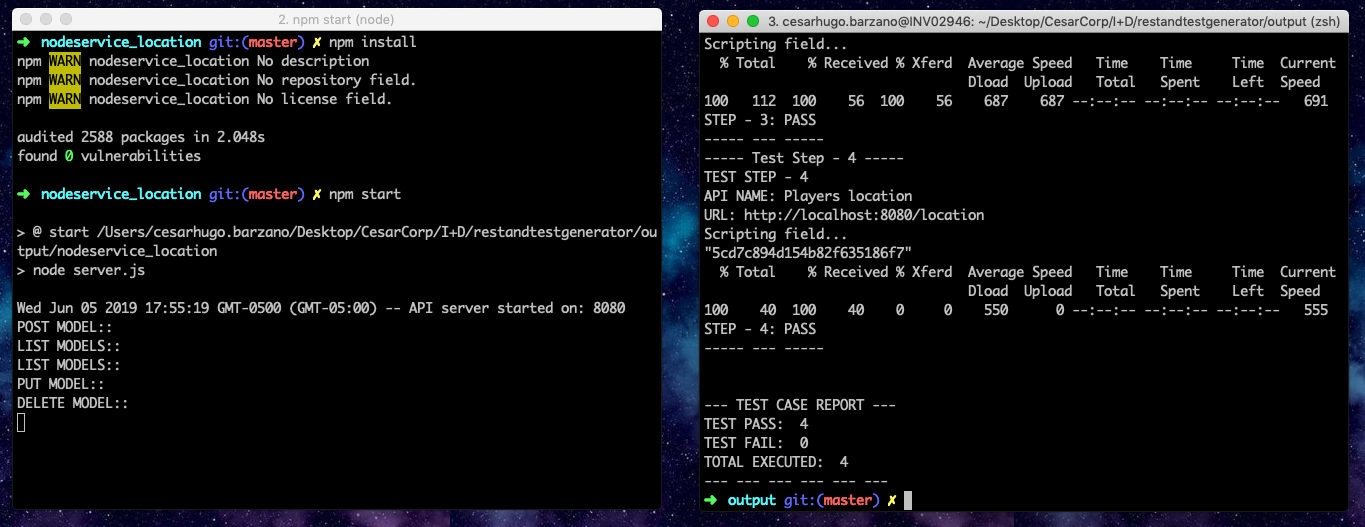
\includegraphics[scale=0.25]{imagenes/t24.png}
\caption{ test\_location.sh result}  
\end{figure}

Es interesante tener en cuenta que los códigos de estado devueltos por el protocolo HTTP son los que marcan el comportamiento de las peticiones atendidas por el servicio web y son usados por el test case para validar el resultado. 

\begin{figure}[H]  
\centering 
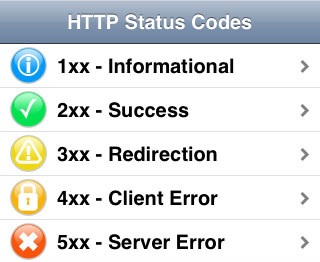
\includegraphics[scale=0.35]{imagenes/http.jpg}
\caption{ HTTP Status Codes}  
\end{figure}

\subsection{Escenario 3: Miauuu as a service}

En este escenario se va ha generar el siguiente servicio:

\begin{lstlisting}[language=python,caption={ cats\_cloud\_service.json }]
[{
  "name": "Miauuu as a service",
  "service": "/cats",
  "url": "http://localhost",
  "port":":8080",
  "body": {
    "name":"Wurst",
    "alias": "Mi bolita gatita bonita, la reina",
    "reina": true,
    "age": 1.5,
    "color": "Negro como mi alma"
  }
}]
\end{lstlisting}

El objetivo de este escenario es mostrar el modelo de negocio generado tanto en GO como en NODE. Para generar el servicio es necesario guardar en el directorio input/ la anterior especificación en un fichero denominado cats\_cloud\_service.json y ejecutar:

\begin{lstlisting}[language=python,caption={ Ejemplo Ejecución Generador: cats\_cloud\_service.json  }]
\$  ./restandtestgenerator.darwin 
\end{lstlisting} 

Dicha ejecución produce el siguiente código: 

\begin{figure}[H]  
\centering 
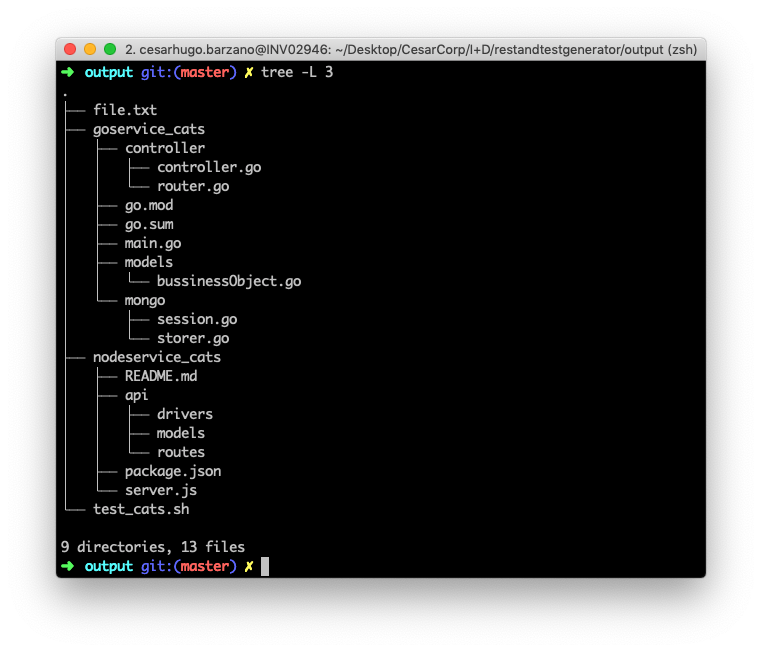
\includegraphics[scale=0.25]{imagenes/t31.png}
\caption{ Servicios /cats generados}  
\end{figure}

Navegando hasta output/goservice\_cats/models/bussinessObject.go se puede observar el modelo de negoció generado para el servicio en GO:

\begin{lstlisting}[language=python,caption={ Ejemplo Modelo de negocio GO  }]
type BusinessObject struct {
	ID     string     	 `bson:"_id" json:"_id,omitempty"`
	Alias    string    `bson:"alias" json:"alias,omitempty"`
	Reina    bool    `bson:"reina" json:"reina,omitempty"`
	Age    float64    `bson:"age" json:"age,omitempty"`
	Color    string    `bson:"color" json:"color,omitempty"`
	Name    string    `bson:"name" json:"name,omitempty"`
}
\end{lstlisting} 

Navegando hasta output/nodeservice\_cats/api/models/backEndModels.js se puede observar el modelo de negoció generado para el servicio en NODE:

\begin{lstlisting}[language=python,caption={  Ejemplo Modelo de negocio NODE }]
var ModelSchema = new Schema ({
  alias : String,
  age : Number,
  color : String,
  name : String,
});
\end{lstlisting} 

\subsection{Escenario 4: Múltiples Servicios}

En este escenario se va a mostrar la capacidad del generador para producir múltiples servicios. Para ello, dentro del directorio input/ se van a guardar las especificaciones de servicio usadas en los ejemplos anteriores junto con la siguiente servicio. Dicho servicio ejemplifica la posibilidad de usar un servicio web para controlar la asistencia de alumnos a cierta asignatura y el uso del tipo de dato boolean. 

\begin{lstlisting}[language=python,caption={  Ejemplo definición servicio class\_attendance.json}]
[{
  "name": "Attendance service",
  "service": "/student",
  "url": "http://localhost",
  "port":":8080",
  "body": {
    "name":"Cesar Hugo",
    "attendance": true
  }
}]
\end{lstlisting} 

El directorio de entrada quedaría con el siguiente ficheros de especificación: 

\begin{figure}[H]  
\centering 
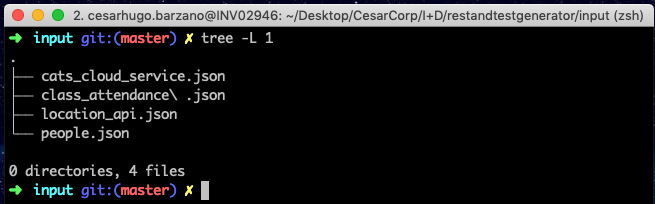
\includegraphics[scale=0.25]{imagenes/t41.png}
\caption{ Múltiples Inputs}  
\end{figure}

Ejecutar el generador: 

\begin{lstlisting}[language=python,caption={ Ejemplo Ejecución Generador: múltiples inputs  }]
\$  ./restandtestgenerator.darwin 
\end{lstlisting} 

Finalmente se genera un servicio NODE, un servicio GO y un caso de prueba.sh para cada uno de los servicios. 

\begin{figure}[H]  
\centering 
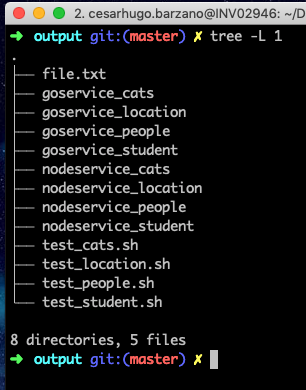
\includegraphics[scale=0.25]{imagenes/t42.png}
\caption{ Múltiples Outputs}  
\end{figure}



\chapter{Entrega}
En este capítulo se detallan cada uno de los ficheros/directorios que forman parte de la entrega. 

\section{Generador}
El generador propuesto por el enunciado se compone de una serie de paquetes GO alojados dentro de testgenerator/src. El generador ha sido desarrollado sobre Ubuntu.18 y hace uso de la versión Go 1.10 pero al ser un lenguaje compilado, podemos elegir entre ejecutar el código fuente ( necesario tener GO instalado en el sistema o utilizar el ejecutable generado con la compilación.  

\section{Makefile}
El fichero ''makefile'' establece las distintas ejecuciones de pruebas para el generador.
 

\section{TI\_CesarHugoBarzanoCruz.pdf}
Memoría de la práctica, referencia a este documento en si mismo, alojado en el directorio raíz de la entrega. 

\section{Directorio DOC}
Directorio donde se almacenan todos los fuentes usados para generar esta documentación utilizando LaTEX. Incluye tambien las imagenes usadas en la memoria. 

\section{Directorio src/testgenerator/input}
Directorio donde se almacenan todos los ficheros usados como configuracion para el generador.

\section{Directorio src/testgenerator/output}
Directorio donde se almacenan todos los ficheros resultados de la ejecución de la pruebas. 

 

\begin{thebibliography}{aaaa}

%intro

\bibitem{go} \textsc{GO},
\textit{The GO Programming Language}
\url{https://golang.org/} 

%Desarrollo

\bibitem{postman} \textsc{Postman},
\textit{POSTMAN API DEVELOPMENT}
\url{https://www.getpostman.com/} 

\bibitem{selenium} \textsc{Selenium},
\textit{Selemium Browser Automation}
\url{https://www.seleniumhq.org/} 

\bibitem{scrum} \textsc{Scrum},
\textit{Scrum Process}
\url{https://winred.es/management/metodologia-scrum-que-es/gmx-niv116-con24594.htm} 

\bibitem{kanban} \textsc{Kanban},
\textit{Kamban Table}
\url{http://www.itmplatform.com/es/blog/kanban-por-que-es-agil-y-en-que-aventaja-a-scrum} 

\bibitem{lean} \textsc{Lean},
\textit{Lean Process}
\url{https://centricconsulting.com/business-consulting/improve-operational-performance/business-process-improvement-lean-six-sigma} 

\bibitem{xp} \textsc{	Kent Beck	},
\textit{Kent Beck - Extreme programming explained: embrace change -Addison-Wesley Longman Publishing Co., Inc. Boston, MA, USA ©2000 ISBN:0-201-61641-6	}
\url{https://dl.acm.org/citation.cfm?id=318762} 

\bibitem{xp2} \textsc{XP},
\textit{Basic Extreme Programming Practices}
\url{https://ronjeffries.com/xprog/what-is-extreme-programming} 


\bibitem{micro} \textsc{Micro-Services ARC},
\textit{Arquitectura basada en microservicios}
\url{https://openwebinars.net/blog/diferencia-entre-arquitectura-monolitica-y-microservicios} 

\bibitem{csp} \textsc{Charles Antony Hoare},
\textit{Communicating sequential processes}
\url{https://www.cs.cmu.edu/~crary/819-f09/Hoare78.pdf}

\bibitem{js} \textsc{JavaScript},
\textit{}
\url{https://www.javascript.com}

\bibitem{node} \textsc{NODE JS},
\textit{JavaScript runtime built on Chrome's V8 JavaScript engine.}
\url{https://nodejs.org/es}

\bibitem{bash} \textsc{Shell BASH},
\textit{Bash Reference Manual}
\url{https://www.gnu.org/software/bash/manual/bash.html}

\bibitem{curl} \textsc{cURL},
\textit{command line tool and library for transferring data with URLs}
\url{https://curl.haxx.se/}



\end{thebibliography}



\chapter{Anexo}





%
%
%%\nocite{*}
%\bibliography{bibliografia/bibliografia}\addcontentsline{toc}{chapter}{Bibliografía}
%\bibliographystyle{miunsrturl}
%
%\appendix

%\input{apendices/manual_usuario/manual_usuario}
%%\input{apendices/paper/paper}
%\input{glosario/entradas_glosario}
% \addcontentsline{toc}{chapter}{Glosario}
% \printglossary

\thispagestyle{empty}

\end{document}
